\documentclass{beamer}
\usepackage{framed}
\usepackage{graphicx}
\usepackage{amsmath}
\usepackage{amssymb}

\begin{document}
\section{Knapsack Problems}
% - https://www.utdallas.edu/~metin/Or6302/Notes/integer.pdf
%- http://www.geeksforgeeks.org/dynamic-programming-set-10-0-1-knapsack-problem/

\begin{frame}
\textbf{The Knapsack Problem}
\begin{figure}
\centering
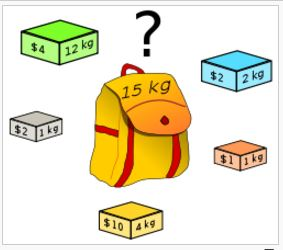
\includegraphics[width=0.7\linewidth]{knapsack}

\end{figure}
\end{frame}
%======================================================= %
\begin{frame}
	\frametitle{The Knapsack Problem}
\Large
\begin{itemize}

\item Given a set of items, each with a weight and a value, determine the number of each item to include in a collection so that the total weight is less than or equal to a given limit and the total value is as large as possible.
\item It derives its name from the problem faced by someone who is constrained by a fixed-size knapsack and must fill it with the most valuable items.
\end{itemize}
	
\end{frame}
%================================= %
\begin{frame}
	\frametitle{Knapsack Problems}
	\Large
	\begin{itemize}
\item The knapsack problem or rucksack problem is a problem in combinatorial optimization.
\item The problem often arises in resource allocation where there are financial constraints and is studied in fields such as combinatorics, computer science, complexity theory, cryptography and applied mathematics.
\end{itemize}

\end{frame}
%================================= %
\begin{frame}
	\frametitle{Knapsack Problems}
	\Large
	\begin{itemize}
\item The knapsack problem has been studied for more than a century, with early works dating as far back as 1897.
\item It is not known how the name "\textit{knapsack problem}" originated, though the problem was referred to as such in the early works of mathematician Tobias Dantzig (1884–1956), suggesting that the name could have existed in folklore before a mathematical problem had been fully defined.

\end{itemize}
\end{frame}

\begin{frame}
	\frametitle{Knapsack Problems}
	\Large
	\begin{itemize}
		\item The most common problem being solved is the \textbf{0-1 knapsack problem}, which restricts the number $x_i$ of copies of each kind of item to zero or one. (i.e. Binary).
		\item Given a set of n items numbered from 1 up to n, each with a weight wi and a value vi, along with a maximum weight capacity W,
	\end{itemize}
	\begin{figure}
		\centering
		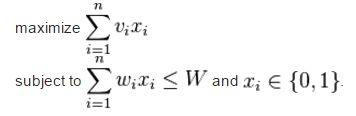
\includegraphics[width=0.7\linewidth]{01knapsack}
	\end{figure}
\textit{(Remark: None or One of each item)}
\end{frame}
%======================================== %
\begin{frame}
	\frametitle{Knapsack Problems}
	\Large
	\begin{itemize}
\item	Here $x_i$ represents the number of instances of item i to include in the knapsack. 
\item Informally, the problem is to maximize the sum of the values of the items in the knapsack so that the sum of the weights is less than or equal to the knapsack's capacity.
	\end{itemize}

\end{frame}
%================================= %
\begin{frame}
	\frametitle{Knapsack Problems}
	\Large
Suppose we have three items as shown in the table below, and suppose the capacity of the knapsack is 5. Formulate the problem.
	\begin{figure}
\centering
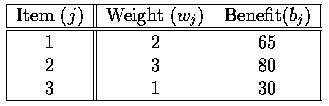
\includegraphics[width=0.7\linewidth]{knapsackexample}
\end{figure}

\end{frame}
%================================= %
\begin{frame}
	\frametitle{Knapsack Problems}
	\Large
	\begin{itemize}
		\item \textbf{Remark:} The 0-1 knapsack problems is an optimization problem.
		\item \textbf{Brute force:} Try all $2^n$ possible subsets (Recall definition of Power Set)
		\item How many combinations if there are 10 items?
		\item	\textbf{Question:} Any solution better than the brute-force?
	\end{itemize}
\end{frame}
%================================= %
\begin{frame}
	\frametitle{Knapsack Problems}
	\Large
	\begin{figure}
\centering
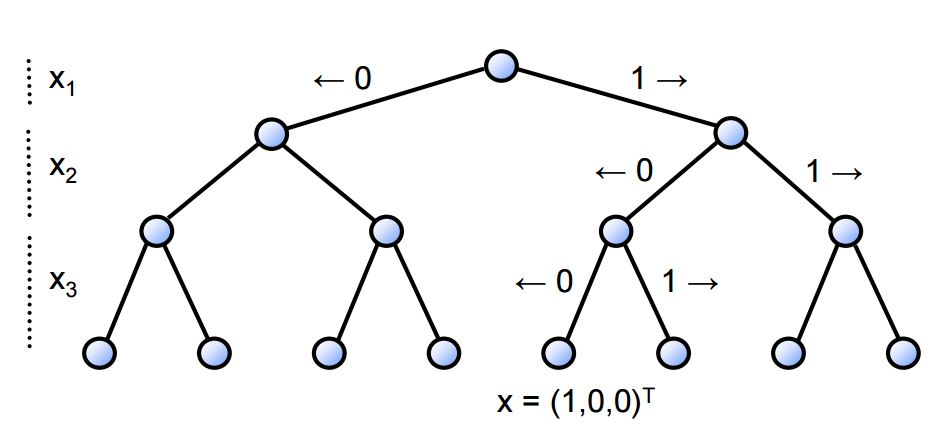
\includegraphics[width=1.1\linewidth]{01knapsack-tree}
\end{figure}

\end{frame}
%================================= %
\begin{frame}
	\frametitle{Knapsack Problems}
	\Large
\noindent \textbf{Branch and Bound}
\begin{itemize}
	\item  Relax the 0/1 integer constraint 
	\item  i.e. Let ``$x_i \in \{0,1\}$" become ``$0\leq x_i \leq 1$".
	\item Branch on the most fractional variable.
\end{itemize}
\end{frame}
%================================================== %
\begin{frame}
	\frametitle{Knapsack Problems}
	\Large
	The \textbf{bounded knapsack problem (BKP)} removes the restriction that there is only one of each item, but restricts the number $x_i$ of copies of each kind of item to an integer value $c_i$:
	\begin{figure}
		\centering
		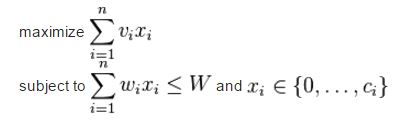
\includegraphics[width=0.7\linewidth]{boundedknapsack}

	\end{figure}
\end{frame}
%================================================= %
\begin{frame}
	\frametitle{Knapsack Problems}
	\Large
	The \textbf{unbounded knapsack problem} \textbf{(UKP)} places no upper bound on the number of copies of each kind of item and can be formulated as above except for that the only restriction on $x_i$ is that it is a non-negative integer.
	\begin{figure}
		\centering
		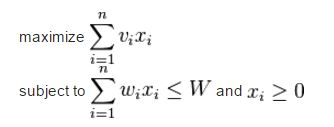
\includegraphics[width=0.7\linewidth]{unboundedknapsack}
	\end{figure}
	
\end{frame}





\end{document}